O \emph{boletim meteorológico diário} do LabInstru é um informativo dos dados registrados pela estação meteorológica da EST/UEA através da utilização de imagens ilustrativas, visando apresentar diferentes aspectos do tempo, tais como: temperatura máxima e mínima, ocorrência ou não de precipitação, velocidade máxima do vento, rajada e índice de calor. Estes boletins são produzidos para divulgação junto à comunidade, como uma maneira resumida de apresentar dados relacionados às variáveis meteorológicas registradas na estação. Exemplos desses boletins meteorológicos produzidos pelo LabInstru podem ser visualizados na Figura \ref{fig:bm}.

\begin{figure}[h!]
	\centering
	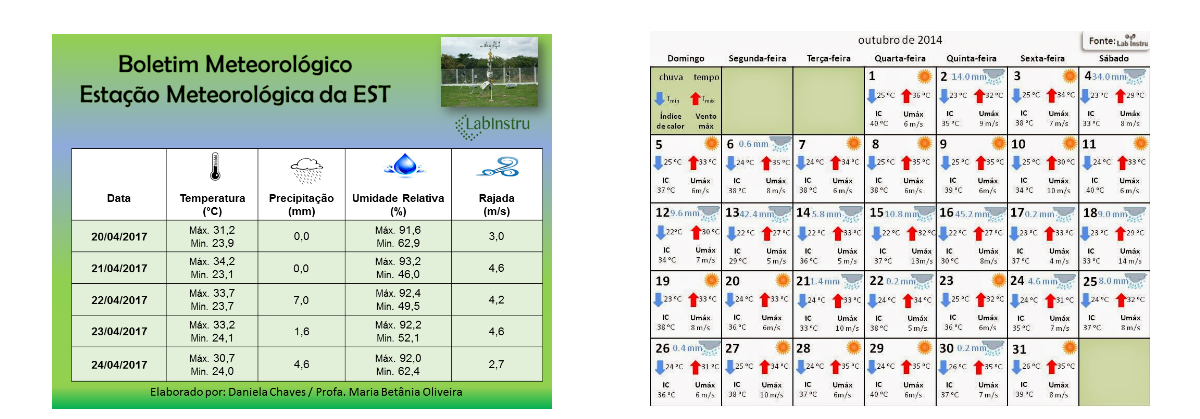
\includegraphics[width=0.9\textwidth]{./img/bm.png}
	\caption{Exemplos de boletins meteorológicos produzidos pelo LabInstru. Fonte: \cite{Labinstru:EST}} \label{fig:bm}
\end{figure}

A produção de boletins meteorológicos é uma das atribuições do LabInstru e pode ser visto como uma forma de fácil assimilação dos dados meteorológicos produzidos pela equipe do laboratório. Considerando a sua importância, um trabalho anterior visou produzir estes boletins de maneira automática através de uma ferramenta intitulada BoCliMa, acrônimo para Boletim Climático de Manaus \cite{Lima:Artigo}.

O BoCliMa produz boletins meteorológicos a partir dos dados da estação meteorológica da EST/UEA, exibindo boletins por turno e diários. Cada boletim contempla a data, ocorrência ou não de precipitação, temperaturas máxima e mínima, índice de calor e rajada de vento, que se caracteriza como a maior velocidade do vento registrada em um dia. Um exemplo de boletim produzido pelo BoCliMa encontra-se ilustrado na Figura \ref{fig:boclima}.

\begin{figure}[h!]
	\centering
	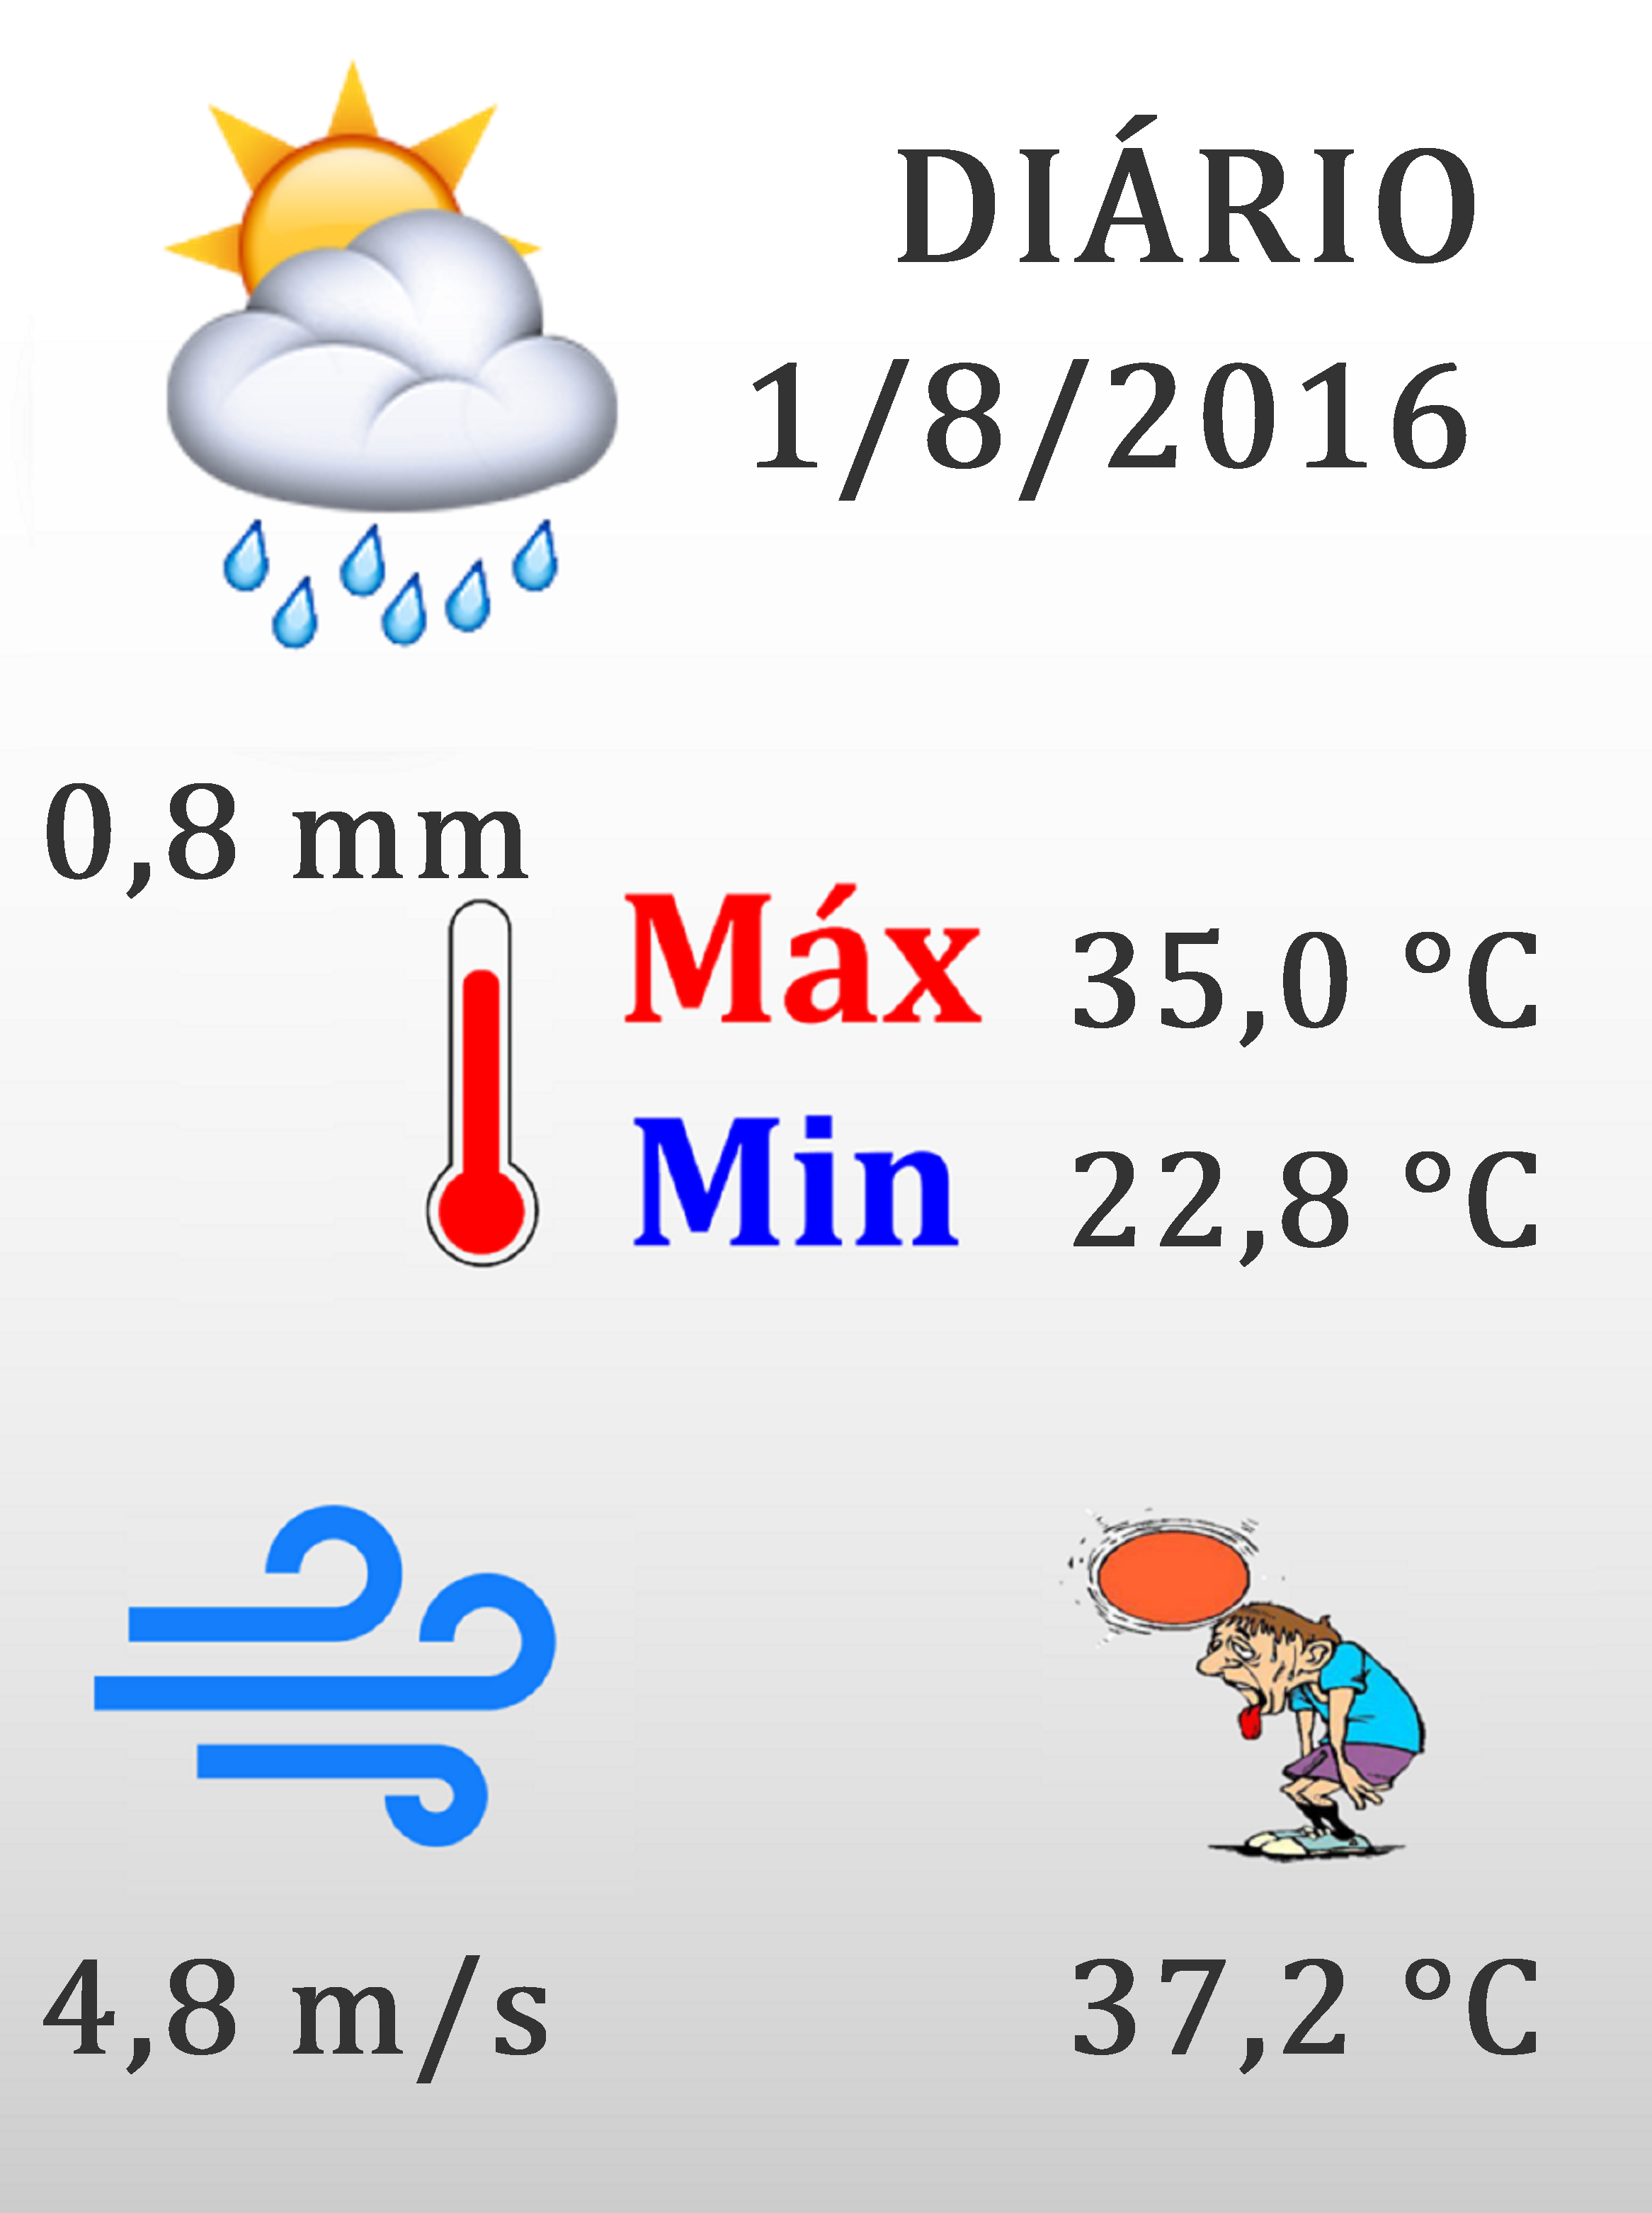
\includegraphics[width=0.3\textwidth]{./img/boclima}
	\caption{Exemplos de boletim meteorológico gerado pelo BoCliMa. } \label{fig:boclima}
\end{figure}

A produção de um boletim meteorológico pelo BoCliMa demanda que o usuário forneça os arquivos com as medições do dia que deseja produzir o boletim. Para tanto, o usuário precisa manualmente consultar os diferentes arquivos produzidos pelas estações e sintetizar um novo arquivo que possa alimentar o BoCliMa. Além destas dificuldades, é possível também observar que no boletim meteorológico produzido, não há uma legenda adequada das informações disponibilizadas (indicando, por exemplo, o índice de calor, as rajadas, etc.) e que também não possui referências ao LabInstru e nem tampouco à cidade de Manaus.

Minimizar as limitações identificadas no boletim produzido pelo BoCliMa e tirar proveito da facilidade de integrar a produção de boletins a uma plataforma que já contempla as medições da estação meteorológica da EST são aspectos que foram considerados no escopo deste trabalho de conclusão de curso, visando prover um melhor suporte na realização das atividades do LabInstru.
